The models, mechanical and computational, were extensively tested in Gazebo. There were a total of three different environments, one for just the vehicle, one for just the arm (mounted to the world), and one with both, where the arm is mounted to the lower portion of the chassis, as seen in Figure~\ref{sample_return_rover:model_validation:combined}. \\

As mentioned before, the models were created in SolidWorks, which is how the render can occur. Furthermore, the kinematic equations were implemented in C++. ROS was utilized to connect the Gazebo joint controllers to the outputs of the various kinematic calculation servers. These files of interest are located in the \ac{SRR} workspace directory as follows:

\begin{itemize}
	\item Arm Forward and Inverse Kinematics Server: ArmKinContainer and ArmKinCalculator in the SRR's kinematics package
	\item Vehicle Velocity Kinematics Server: VehicleVelKinContainer and VehicleVelKinCalculator in the SRR's kinematics package
	\item Combined Inverse Kinematics Server: CombinedKinContainer and CombinedKinCalculator in the SRR's kinematics package
\end{itemize}

\begin{figure}[H]
	\centering
	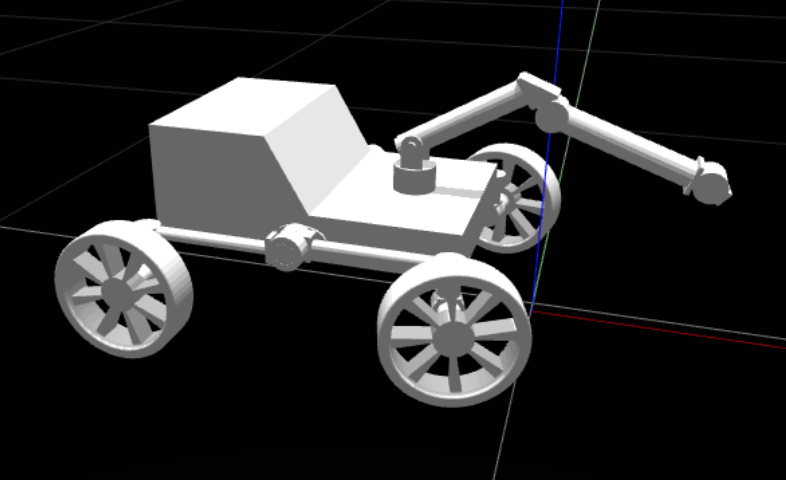
\includegraphics[width=\textwidth]{sections/robot-design/images/combined_sim.png}
	\caption{Gazebo Simulation of the Combined Vehicle and Arm Models}
	\label{sample_return_rover:model_validation:combined}
\end{figure}
